% !TeX spellcheck = en_US
%===============================================================================
% $Id: ifacconf.tex 19 2011-10-27 09:32:13Z jpuente $
% Template for IFAC meeting papers
% Copyright (c) 2007-2008 International Federation of Automatic Control
%===============================================================================
\documentclass{ifacconf}

\usepackage{graphicx}      % include this line if your document contains figures
\usepackage{natbib}        % required for bibliography

\usepackage[utf8]{inputenc}

\usepackage{amsmath}
\usepackage{amssymb}
\usepackage{color}
\usepackage{datetime}

%===============================================================================

\graphicspath{
{images/}
}

% Custom commands
\providecommand{\mbf}[1]{\mathbf{#1}}
\newcommand{\idxFollower}{{\ensuremath{i} }}
\newcommand{\idxPredecessor}{{\ensuremath{i-1} }}
\newcommand{\idxSample}{{\ensuremath{k}}}
\newcommand{\idxAxis}{{\ensuremath{p}}}

\begin{document}
\begin{frontmatter}

\title{Discrete Sliding Mode control of small UAS in tight formation flight under information constraints}
% Title, preferably not more than 10 words.

\author[First]{Jan Bolting}
\author[Second]{Soheib Fergani}
\author[Third]{Jean-Marc Biannic}
\author[Fourth]{Francois Defay}
\author[Fifth]{Martin Stolle}

\address[First]{National Institute of Standards and Technology,
   Boulder, CO 80305 USA (e-mail: author@ boulder.nist.gov).}
\address[Second]{Colorado State University,
   Fort Collins, CO 80523 USA (e-mail: author@lamar. colostate.edu)}
\address[Third]{Electrical Engineering Department,
   Seoul National University, Seoul, Korea, (e-mail: author@snu.ac.kr)}

\textcolor{red}{\Huge !!! DRAFT !!!\\ \normalsize \today \\ \currenttime}

% Abstract of not more than 250 words.
\begin{abstract}
This papers is concerned with a new control strategy  based on discrete sliding mode control of small Unmanned Aerial Systems (UAS) in tight formation flight under information constraints. It addresses the problem of managing and coordinating several UAS to fly in a tight control formation. Since the formation of $n$ UAS to be controlled is considered to fly in an arbitrary pattern in this work, a high-performance relative position control becomes an important issue. Indeed, a robust control strategy based on the sliding mode approach is proposed to achieve the desired flight performances while assuming realistic information constraints imposed by limited communication bandwidth and availability of relative localization sensors and preserving scalability with respect to formation size.\\
Also, this paper presents a meaningful study and comparison of the discrete sliding mode control design (DSMC) and  time sampling continuous sliding mode control (TSCSMC). Indeed, it is important to study the performance differences between the two approaches that allow to choose the best strategy to be used to solve the considered problem. Here, the comparison focuses on the effect of the sampling on the control error, the mesh stability analytically and the mesh stability in simulation.\\

Simulation results of a flight scenario with two different sampling frequencies proves the efficiency of the proposed control strategy and shows clearly the effect of the discretization and the sampling  on the formation flight behaviour of the UAS obtained by the chosen considered control.


%Indeed, the capability of autonomous formation flight has the potential to significantly enhance the utility and efficiency of small low-cost UAS. Formations of small, inexpensive fixed-wing UAS allow for the sharing of remote sensing functionality, mission-level redundancy and range enhancements due to aerodynamic interactions widely exploited by migratory birds.
%
%The capability of autonomous formation flight has the potential to significantly enhance the utility and efficiency of small low-cost Unmanned Aerial Systems (UAS). Formations of small, inexpensive fixed-wing UAS allow for the sharing of remote sensing functionality, mission-level redundancy and range enhancements due to aerodynamic interactions widely exploited by migratory birds.
%For the latter application, high-performance relative position control is essential.
%This becomes challenging when assuming realistic information constraints imposed by limited communication bandwidth and availability of relative localization sensors,  while preserving scalability with respect to formation size.
%This article presents a Discrete Time Sliding Mode controller for tight formation flight and studies its
%
%State-based STCSMC\\
%State-based DSMC\\
%For both:\\
%Effects of sampling on control error\\
%Effects of sampling on mesh stability in simulation\\
%Effects of sampling on mesh stability analytically
\end{abstract}

\begin{keyword}
Flight formation, Aerospace unmanned vehicle, sliding mode control.
\end{keyword}

\end{frontmatter}
%===============================================================================

\section{Introduction}

The capability of autonomous formation flight has the potential to significantly enhance the utility and efficiency of small low-cost UAS. Formations of small, inexpensive fixed-wing UAS allow for the sharing of remote sensing functionality, mission-level redundancy and range enhancements due to aerodynamic interactions widely exploited by migratory birds. Indeed, aircraft's formation flight can enhance the fuel efficiency thanks to the aerodynamics and the induced airflow by leading aircraft, in the same way that the migratory birds use some formation patterns. Indeed, in \cite{weimerskirch2001energy} authors  have measured heart rates as an estimate of energy expenditure in imprinted great white pelicans (Pelecanus onocrotalus) trained to fly in 'V' formation, and show that these birds save a significant amount of energy by flying in formation. This advantage is probably a principal reason for the evolution of flight formation in large birds that migrate in groups.\\
 Also, this strategy has a lot of advantages as sharing of remote sensing functionality, mission-level redundancy, range enhancements due to aerodynamic interactions and energy saving. Based on that, the NASA AFF program has demonstrated the feasibility of this approach for manned fighter aircraft in a 2-aircraft configuration. Maximum fuel savings of $14\%$ for the follower are reported. This emphasize on the importance of the flight formation since no structural changes have to be made to the aircraft to gain considerable fuel savings.\\

Recently, both academical and industrial communities have been very interested in the flight formation of aircrafts and UAS. In \cite{wolfe1996decentralized}, decentralized control is presented to increase the efficiency of flight formation of $5$ aircraft in a single line. These controllers are derived from a linear model and tested on a linear simulation incorporating a vortex-latting aerodynamics routine. Another interesting study in \cite{thien2008effects} focuses on the effect of its position and shape on aerodynamics performances of a given V flight formation. Vortices generated the wing tip of the leader moves downstream forming a pair of opposite rotating line vortices. Some interesting control solutions for autonomous flight formation were introduced in \cite{giulietti2000autonomous}. Moreover, in the last decade, a lot of researchers have focused on improving the control strategies to enhance the formation flight performance behaviour. A suitable control strategy for  controlling a team of micro-aerial vehicles moving quickly through a three-dimensional environment while maintaining a tight formation is presented in \cite{turpin2012trajectory}. Moreover, an interesting control performance analysis for autonomous close formation flight experiments has been achieved in \cite{rice2014control}.\\
In this paper, a discrete robust sliding mode control strategy is proposed to manage the formation flight of UAS. Indeed, sliding mode control has been proved as a very efficient implementable solution for ground vehicle platooning (see \cite{ferrara2008sliding} and \cite{zou2013distributed}). Also, the sliding mode control is very efficient and robust approach regarding environmental disturbances to ensure a good position tracking performances. Here, authors provide a robust discrete sliding mode control solution to manage the tight formation flight of the UAS considering external disturbances. Then, a comparison between the discrete time sliding monde control design and the discretization of a time continuous sliding mode control is achieved. Indeed, it proves that the discretization of the time continuous designed controller decreases the tracking performances and the robustness regarding the environmental disturbances.\\
This paper is structured as follows: section...


\section{Model}

\subsection{Coordinate frames}
The system to be controlled is a formation of $n$ UAS flying in an arbitrary pattern. Is is assumed that
load factors are controlled in each vehicle's body frame (index $b$). Therefore separation errors are transformed into the body frame for control purposes, decoupling the three axes. The dynamics of each vehicle are defined in a local inertial North-East-Down frame (index $e$).

%The right choice of reference frames can significantly facilitate control design. To give one example, when performing navigation in the predecessor's body frame, variations in the predecessor's attitude will couple into follower's position control loops, increasing control action. What is more, the effect increases with inter-vehicle separation, leading to high control demands during the initial rendezvous maneuver. To avoid such disadvantages, the motion of the reference frame with respect to the inertial frame should be within the control bandwidth of the position controller. A suitable frame is a local Cartesian frame whose x axis is aligned with the follower's inertial speed projected on the horizontal plane, and whose z axis is aligned with the NED frame's z axis, the Follower Velocity Frame (FF). Its origin coincides with that of the follower's body frame. The follower's wind frame would be preferable, since the lift vector is by definition aligned with its z axis , but requires on-line wind estimation or flow sensors that usually are not available on board small UAS. It is preferable over the Predecessor Velocity Frame (PF), since to form the rotation matrix between the FF and the inertial frame the predecessor's absolute velocity does not need to be communicated to the follower.

To dispose of a common reference frame for multiple members of the formation, the \textbf{Leader Speed Frame} (index $ls$) is defined. Its x axis is aligned with the formation leader's NED speed projected on the horizontal plane, its z axis is aligned with the NED frame's z axis, and its y axis completes a right-handed Cartesian coordinate system. I is used to define the separation vectors that make up the formation.

\begin{figure}
\begin{center}
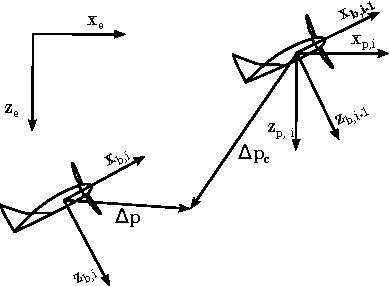
\includegraphics[width=8.4cm]{frames}    % The printed column width is 8.4 cm.
\caption{Predecessor-follower geometry longitudinal}
\label{fig:frames}
\end{center}
\end{figure}

\subsection{Vehicle Model}

The continuous time vehicle position dynamics w.r.t. the local inertial frame are given by

\begin{align}
\mathbf{x} &= (\mbf{p} \; \mbf{v})^T \\
\dot{\mathbf{p}} &= \mbf{v}\\
\dot{\mbf{v}} &= \mbf{a}_{c} + \mbf{a}_w + \mbf{g}
\end{align}

where $\mbf{p} \in \mathbb{R}^3$ is the vehicle position, $\mbf{v} \in \mathbb{R}^3$ is its velocity w.r.t to the local inertial frame, $\mbf{a}_w \in \mathbb{R}^3$ are accelerations induced by exogenous disturbances such as turbulence and another aircraft's wake, $\mbf{a}_{c} \in \mathbb{R}^3$ are commanded accelerations and $\mbf{g} \in \mathbb{R}^3$ is the gravity vector in the local inertial frame.

It is assumed that load factors $\mbf{n}_c$ are tracked by fast inner loop controllers in the vehicle body frame, leading to actual load factors $\mbf{n} = \mbf{n}_c + \mbf{n}_w$ where $\mbf{n}_w = \frac{1}{|\mbf{g}|} \mbf{a}_w$ are parasitic load factors introduced by exogenous disturbances and imperfect tracking. This leads to

\begin{align}
\dot{\mbf{v}} &= \mbf{R}_{eb} |\mbf{g}|\mbf{n}_c + \mbf{a}_w + \mbf{g}
\label{eq:svmloadfactorlevel}
\end{align}

where $\mbf{R}_{eb} \in \mathbb{R}^{3 \times 3}$ is the rotation matrix from the body frame to the local inertial frame and $\mbf{n}_c = \frac{1}{|\mbf{g}|} \mbf{a}_c$ are commanded load factors. To simplify notation, is is assumed that the vehicle is trimmed, i.e. the nominal gravitational acceleration is compensated for by a trim control input $\mbf{n}_{c,0} = \mbf{R}_{be}(0 \; 0 \; -1)^{T}$ and a virtual control input is defined as

\begin{align}
\mbf{u} = \mbf{R}_{eb} |\mbf{g}|(\mbf{n}_c - \mbf{n}_{c,0})	
\label{eq:defushort}
\end{align}

leading to

\begin{align}
\dot{\mbf{v}} &= \mbf{R}_{eb}|\mbf{g}|
(
\frac{1}{|\mbf{g}|}
(\mbf{R}_{be} \mbf{u} + \mbf{n}_{c,0})
) + \mbf{a}_w + \mbf{g}\\
\dot{\mbf{v}} &= \mbf{u} + \mbf{a}_w
\label{eq:svmshort}
\end{align}

where now $\mbf{a}_w$ also includes the small effects of imperfect knowledge of local gravitation. ???doubledefinition

Saturations on the virtual control input (\ref{eq:defu}) can be derived from (\ref{eq:loadfactorsaturations}) as

\begin{align}
|\mbf{u}| &\leq \mbf{U} \\
\mbf{U} &= \mbf{R}_{eb} |\mbf{g}|(\mbf{N}-\mbf{n}_{c,0})
\end{align}


Considering two UAS \idxFollower  and \idxPredecessor, this leads to relative position error dynamics

\begin{align}
\Delta \mbf{p} &= \mbf{p}_\idxFollower - \mbf{p}_\idxPredecessor - \Delta \mbf{p}_c \\
\Delta \dot{\mbf{p}} &= \mbf{v}_{\idxFollower} - \mbf{v}_{\idxPredecessor} -  \Delta \dot{\mbf{p}}_c\\
\Delta \dot{\mbf{v}} &= \mbf{a}_\idxFollower - \mbf{a}_\idxPredecessor -  \Delta \ddot{\mbf{p}}_c\\
{} &= \mbf{a}_{c,\idxFollower} + \mbf{a}_{w,\idxFollower}
 - \mbf{a}_\idxPredecessor -  \Delta \ddot{\mbf{p}}_c\\
{} &= \mbf{u} + \mbf{a}_{w,\idxFollower}
 - \mbf{a}_\idxPredecessor -  \Delta \ddot{\mbf{p}}_c
\end{align}

where $\Delta \mbf{p}$ is the relative position error between UAS \idxFollower and its predecessor \idxPredecessor, $\Delta \mbf{v}$ is the corresponding relative velocity error, $\Delta \mbf{p}_c$ is the desired relative position to the predecessor, $\mbf{a}$ are accelerations.

The presented model is essentially of the same type as that used in  \cite{galzi2006uav} and provides the benefit of being vehicle-agnostic, as the specific vehicle dynamics are covered by the inner loop load factor controllers. On the other hand, perturbations $\mbf{a}_w$ and control input saturations are specific to a given vehicle and mission environment. It covers rotary wings as well as fixed wing UAS, which are the focus of this work.

\subsubsection{Formation geometry}
The trajectory of the formation w.r.t. the local inertial frame is defined by the nominal trajectory of a virtual leader aircraft. Arbitrary shapes of the formation can be defined by the relative separation vectors $\Delta \mbf{p}$. 

\section{Control design}
To benefit from significant aerodynamic performance gains, a follower aircraft needs to stay within a narrow spatial window roughly defined by (see e.g. \cite{jake2003f})

{\centering
$-0.2 b < \Delta y' < -0.1 b$ \\
$-0.1 b < \Delta z' < 0$ \\
}

while the longitudinal separation $\Delta x'$ is less critical due to slow vortex decay.
It is thus the control objective to drive the follower UAS into this window and stay within in.

\subsection{Input saturations}
For a fixed-wing UAS, the maximum load factors are naturally limited by the maximum thrust of the engine and the aerodynamic parameters of the aircraft, such as the stall angle $\alpha_{max}$ as

\begin{align}
|\mbf{n}(t)| \leq \mbf{N}(t)
\label{eq:loadfactorsaturations}
\end{align}

These saturations are time-varying since, including the engine thrust, they are function of the dynamic pressure $\bar{q}(t) = \frac{1}{2}\rho(t) V_a^2(t)$.

\subsection{Information constraints}
It is assumed that observations of the relative position and relative velocity vector between each UAS and its predecessor are available.

This limitation allows to use low-cost vision-based relative localization techniques, which is a significant advantage taking into account the price range of GNSS Real Time Kinematics systems which would be required for localization with respect to the formation leader or other members of the formation that are now within the field of view of onboard vision sensors.

\begin{figure}
\begin{center}
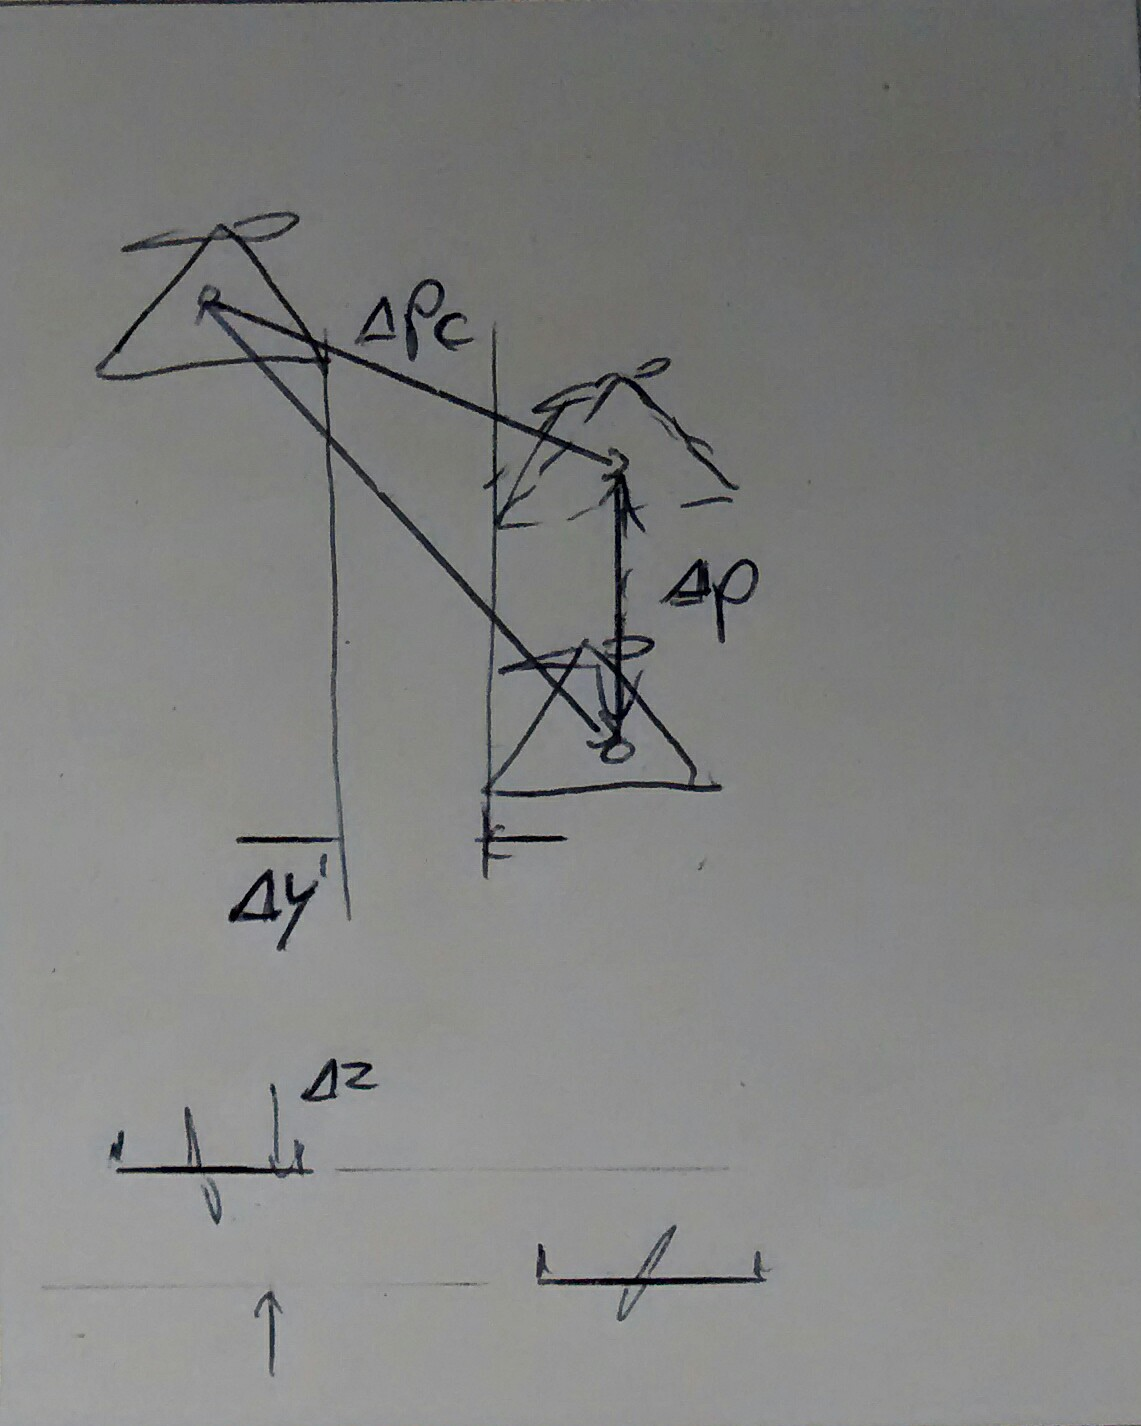
\includegraphics[width=8.4cm]{geometry}    % The printed column width is 8.4 cm.
\caption{Predecessor-follower geometry}
\label{fig:geometry}
\end{center}
\end{figure}

\subsection{CSMC}

It is the control objective to drive the system to the sliding surface defined by

\begin{align}
\mbf{\sigma}(t) &= \mbf{G}\mbf{x}(t)
\label{eq:defsigmaconti-} \\
\mbf{x}(t) &=
\begin{pmatrix}
\Delta \mbf{p}(t)\\
\Delta \mbf{v}(t)
\end{pmatrix}
\end{align}

and, once reached, to keep it on it for all subsequent times $t \geq t^*$. With

\begin{align}
\mbf{G} =
\begin{bmatrix}
\mbf{G}_1 \mbf{G}_2
\end{bmatrix}
\end{align}

the position error dynamics in sliding mode are

\begin{align}
\mbf{0}
&=
\begin{bmatrix}
\mbf{G}_1 \mbf{G}_2
\end{bmatrix}
\begin{pmatrix}
\Delta \mbf{p}(t)\\
\Delta \mbf{v}(t)
\end{pmatrix} \\
\mbf{\Delta} \dot{\mbf{p}}
&= - \mbf{G}_2^{-1} \mbf{G}_1 \mbf{\Delta} \mbf{p}
\label{eq:pdynwhilesliding}
\end{align}

Selecting $- \mbf{G}_2^{-1} \mbf{G}_1$ as Hurwitz ensures that $\Delta \mbf{p}$ asymptotically converges to zero while in sliding mode.

Mesh stability is a feature of a three-dimensional formation of vehicles that allows separation errors to stay locally contained (see e.g. \cite{Pant2002}). In other words, separation errors between a pair of vehicles are not amplified towards the neighboring vehicle pairs. More vehicles can be added to a mesh stable formation without changing the local controllers, providing scalability. It is a well known fact (\cite{Pant2002}) that linear controllers with local feedback information are mesh unstable.

While in sliding mode, the position error dynamics are by definition confined to (\ref{eq:pdynwhilesliding}), independently of adjacent separation errors, implying mesh stability if the system can be kept in sliding mode.

The open loop sliding variable dynamics are

\begin{align}
\dot{{\sigma}} &= \mbf{G}
\begin{pmatrix}
\Delta \mbf{v} \\
\mbf{u} + \mbf{a}_{w,\idxFollower}
 - \mbf{a}_\idxPredecessor -  \Delta \ddot{\mbf{p}}_c
\end{pmatrix}\\
& = \mbf{G}
\begin{pmatrix}
\Delta \mbf{v} \\
 - \Delta \ddot{\mbf{p}}_c
\end{pmatrix} 
+ \mbf{G}
\begin{bmatrix}
{\mbf{0}}\\
{\mbf{I}}
\end{bmatrix}
(\mbf{u} + \mbf{a}_{w,\idxFollower} + \mbf{a}_\idxPredecessor) \\
&= \mbf{G} \mbf{\Phi}_k + \mbf{G} \mbf{B}(
\mbf{u}
 + {\mbf\Phi}_u)
\label{eq:sigmadynconti}\\
&= \mbf{\Phi}'_k + \mbf{\Phi}'_u + \mbf{u}'
\label{eq:sigmadyncontishort}
\end{align}

The  desired relative position $\Delta \mbf{p}_c$ and its second derivative are communicated to each follower. Accelerations of the predecessor $\mbf{a}_{k-1}$ as well as exogenous perturbations $\mbf{a}_w $ acting on the vehicle $i$ are assumed to be unknown but bounded. For notational convenience they are lumped into the disturbance vector $\mbf{\Phi}_u$

\begin{align}
\mbf{\Phi}_u &= \mbf{a}_{w,\idxFollower} - \mbf{a}_\idxPredecessor
\end{align}

while the known perturbations $\Delta \ddot{\mbf{p}}_c$ are redefined as $\mbf{\Phi}_k$

\begin{align}
\mbf{\Phi}_k &= 
\begin{pmatrix}
\Delta \mbf{v} \\
 - \Delta \ddot{\mbf{p}}_c
\end{pmatrix} 
\end{align}

further defining

\begin{align}
\mbf{u}' &= \mbf{GB}\mbf{u}
\label{eq:defu}\\
\mbf{\Phi}_k' &= \mbf{G}\mbf{\Phi}_k \\
\mbf{\Phi}_u' &= \mbf{GB}\mbf{\Phi}_u
\end{align}

Note that all perturbations are assumed to satisfy the matching condition.
The three axes are considered decoupled by the inner load factor controllers, allowing for SISO design.

Saturations on the virtual control input (\ref{eq:defu}) can be derived from (\ref{eq:loadfactorsaturations}) as

\begin{align}
|\mbf{u}'| &\leq \mbf{U}' \\
\mbf{U}' &= \mbf{GB} \mbf{R}_{eb} |\mbf{g}|(\mbf{N}-\mbf{n}_{c,0})
\end{align}

Since the inner loop load factor controllers cannot track discontinuous reference signals, a continuous control signal is mandatory.
The system (\ref{eq:sigmadynconti}) is of relative degree $\mbf{r} = (1 \; 1 \; 1)^T$, thus continuous-time Super-Twisting Sliding Mode controllers (CSTSMC, see e.g. \cite{shtessel2014sliding}) can be applied, providing continuous control signals.
We apply the controller presented in \cite{galzi2006uav} extending it trivially from 2D to 3D tracking.
The CSTSMC controller is then given by

\begin{align}
u_\idxAxis' = \alpha_\idxAxis |\sigma_\idxAxis|^{1/2}\mathrm{sign(\sigma_\idxAxis)} + \beta_\idxAxis \int \mathrm{sign}(\sigma_\idxAxis) dt
\end{align}

where $\idxAxis = 1...3$ indicates the three decoupled axes. Adding a term that eliminates the known disturbances ${\Phi}_{k,i}'$ as in \cite{galzi2006uav}

\begin{align}
u_\idxAxis' = \alpha_\idxAxis |\sigma_\idxAxis|^{1/2}\mathrm{sign(\sigma_\idxAxis)} + \beta_\idxAxis \int \mathrm{sign}(\sigma_\idxAxis) dt - {\Phi}'_{k,\idxAxis}
\end{align}

leads to closed loop $\mbf{\sigma}$ dynamics of

\begin{align}
\dot{\sigma}_\idxAxis = \alpha_\idxAxis |\sigma_\idxAxis|^{1/2}\mathrm{sign(\sigma_\idxAxis)} + \beta_\idxAxis \int \mathrm{sign}(\sigma_\idxAxis) dt + \Phi_{u,\idxAxis}'
\end{align}

Provided the disturbances $\Phi'_{u,\idxAxis}$ are bounded by $\Phi'_{u,\idxAxis} \leq L_\idxAxis$ controller parameters that fulfill
\begin{align}
\alpha_\idxAxis = 1.5 \sqrt{L_\idxAxis}
\label{eq:csmcgainconditionalpha}\\
\beta_\idxAxis = 1.1 L_\idxAxis
\label{eq:csmcgainconditionbeta}
\end{align}

 drive the system into 2-sliding mode, i.e. $\dot{\sigma} = \sigma = 0$ in finite time. The reaching time is bounded by $t_\idxAxis^* \leq \frac{7.6 \sigma_\idxAxis(0)}{\beta_\idxAxis - L_\idxAxis}$, see \cite{galzi2006uav}.

The actual control input $\mbf{n}_c$ is computed from (\ref{eq:defu}, \ref{eq:defushort}) as

\begin{align}
\mbf{n}_c = \frac{1}{|\mbf{g}|} \mbf{R}_{be}(\mbf{GB})^{-1} \mbf{u}' + \mbf{n}_{c,0}
\end{align}

using $\mbf{R}_{eb}^{-1} = \mbf{R}_{eb}^{T} = \mbf{R}_{be}$

%\subsubsection{Sliding condition}
%
%Ideal sliding mode controllers completely eliminate the impact of matched perturbations by injecting a control input that perfectly follows them. To verify that the system can actually be kept in sliding mode after the reaching phase despite limited control resources, the equivalent control is computed, i.e. the control that would satisfy the sliding condition if unknown perturbations were known. For (\ref{eq:sigmadyncontishort}), it results to
%
%\begin{align}
%{u}_{eq,i} = - {\Phi}_{k,i}' - {\Phi}_{u,i}'
%\end{align}
%
%Provided that
%\begin{align}
%\mbf{\Phi}_k'
%&= \mbf{G}
%\begin{pmatrix}
%\Delta \mbf{v} \\
% \Delta \ddot{p}_c
%\end{pmatrix}
%&\leq
%\mbf{M}\\
% &{\Phi}_{k,i}'
% &\leq
%{M}_i
%\end{align}
%
%with $\mbf{M} \in \mathbb{R}^3$ and $i=1...3$, $u_{eq,i}$ is bounded by
%
%\begin{align}
%|u_{eq,i}| \leq M_i + L_i
%\end{align}
%
%The unknown perturbations $\Phi_{u,i}$ are driven by exogenous disturbances $a_{w,i}$ and acceleration of the predecessor $a_{k-1,i}$.
%
%!!!Finish equivalent control part

%Those being bounded by (see (\ref{eq:svmloadfactorlevel}))
%
%\begin{align}
%|a_{w,i}| &\leq A_{w,i} \\
%|a_{k-1,i}| &\leq ||\mbf{g}|\mbf{n}_c| + |\mbf{a}_w| + |\mbf{g}|
%\end{align}

%\begin{align}
%u_i &= u_1 +  u_2
%\label{eq:STSMC}\\
%\dot{u}_1 &=
%\begin{array}{lr}
%-u \hspace{2em}
%& \mathrm{if} \; |u| > U\\
%-\alpha \mathrm{sign}(\sigma) \hspace{2em}
%& \mathrm{if} \; |u| \leq U\\
%\end{array} \\
%{u}_2 &=
%\begin{array}{lr}
%-\lambda |\sigma_0|^{1/2} \mathrm{sign}(\sigma)
% \hspace{2em}
%& \mathrm{if} \; |\sigma| > \sigma_0\\
%-\lambda |\sigma|^{1/2} \mathrm{sign}(\sigma)
% \hspace{2em}
%& \mathrm{if} \; |\sigma| \leq \sigma_0\\
%\end{array}
%\end{align}

\subsubsection{Discretization}
For implementation, the CSTSMC is sampled with a zero-order hold scheme. There are results for homogeneous sliding controllers such as the CSTSMC (see \cite{shtessel2014sliding}) stating that the error introduced by discrete sampling is quadratically proportional to the sampling time, i.e. $\sigma = O(T^2)$. Our simulation results confirm this, see section \ref{sec:simulations}.

%\begin{align}
%u_i(\idxSample) = \alpha_i |\sigma_i(\idxSample)|^{1/2}\mathrm{sign(\sigma_i(\idxSample))} + \beta_i
%T
%\sum_{p=0}^{k}
%\mathrm{sign}(\sigma_i(p))
%\end{align}

\subsection{DSMC}
Designing a sliding mode controller in the discrete time domain allows to take sampling time effects into account right from the beginning. \\
The $\sigma$ dynamics assuming forward Euler discretization are

\begin{align}
{{\sigma}}(\idxSample+1)
&=
{{\sigma}}(\idxSample)
+
T(
\mbf{\Phi}'_k(\idxSample) + \mbf{\Phi}'_u(\idxSample) + \mbf{u}'(\idxSample))
\label{eq:sigmadyndiscrete}
\end{align}

Since a discrete controller has no control over what happens to the continuous system between sampling instants, ideal sliding mode is not achievable. It is however possible to drive the system into so-called quasi-sliding mode, defined by the control objective

\begin{align}
|{\sigma}_i(\idxSample)| \leq \mbf{\epsilon}_i
\label{eq:controlobjective}
\end{align}

for $i=1...3$, for all $k \geq k^*$ where $\epsilon$ is the width of the quasi-sliding mode boundary layer and $k^*$ is the first sample for which eq. \ref{eq:controlobjective} is satisfied, i.e. when the system transitions from the reaching phase into quasi-sliding mode.
The proposed DSMC is based on ideas presented by the authors of \cite{monsees2001discrete}
The following simple linear reaching law (proposed e.g. by \cite{Spurgeon1992}) ensures asymptotic convergence to the sliding surface

\begin{align}
\mbf{\sigma}(\idxSample+1) = \mbf{\Psi} \mbf{\sigma}(\idxSample)
\label{eq:reachinglaw}
\end{align}

with a diagonal $\mbf{\Psi} \in \mathbb{R}^{3 \times 3}, 0 < \Psi_{i,i} < 1$ for $i=1...3$. The choice of $\mbf{\Psi}$ allows to trade off control effort and reaching time.
Since (\ref{eq:reachinglaw}) is equivalent to

\begin{align}
|\mbf{\sigma}(\idxSample+1)| = \mbf{\Psi} |\mbf{\sigma}(\idxSample)|
\end{align}

the norm of the sliding variable decreases with every time step, indicating convergence to the sliding surface. 

\subsubsection{Remark} As mentioned in \cite{monsees2001discrete}, a Lyapunov function does not - as in the continuous case - provide enough constraints to drive the system to the sliding surface without overshoot. This is due to the fact that a Lyapunov function only constrains the direction of the system's motion - towards the sliding surface - but not the magnitude of the next discrete step towards it. 

The control input $\mbf{u}(\idxSample)$ required to drive the system (\ref{eq:sigmadyndiscrete}) according to the reaching law (\ref{eq:reachinglaw}) can be computed from the open-loop $\mbf{\sigma}$ dynamics to

\begin{align}
\mbf{u}'(\idxSample) &= \frac{1}{T}(\mbf{\Psi} - \mbf{I})\mbf{\sigma}(\idxSample) - \mbf{\Phi}_k' - \tilde{\mbf{\Phi}}_u'
\end{align}

Note that $\mbf{u}'(\idxSample)$ contains an estimate of the unknown perturbations $\tilde{\mbf{\Phi}}'_u(\idxSample) = \mbf{\Phi}'_u(\idxSample) + \Delta \mbf{\Phi}'_u(\idxSample)$. Closing the loop, one obtains

\begin{align}
\mbf{\sigma}(\idxSample+1) &= \mbf{\Psi} \mbf{\sigma}(\idxSample) +
T (\Delta \mbf{\Phi}'_u(\idxSample))
\end{align}

Note that the reaching law (\ref{eq:reachinglaw}) can not be followed due to the estimation error $\Delta \mbf{\Phi}'_u(\idxSample)$. Instead, assuming that initially the system is outside the quasi-sliding mode band, it will approach the sliding surface at least as long as

\begin{align}
\mbf{\Psi} \mbf{\sigma}(\idxSample) & \geq T (\Delta \mbf{\Phi}_u(\idxSample))
\end{align}

This defines the maximum boundary layer thickness as

\begin{align}
\epsilon &=
\mbf{\Psi}^{-1} T (\Delta \mbf{\Phi}_u(\idxSample))
\label{eq:achievableepsilon}
\end{align}

%To verify that once inside the boundary layer, the system stays in it, consider
%
%\begin{align}
%
%\end{align}
%
%Note that with a diagonal $\mbf{\Psi} \in \mathbb{R}^{3 \times 3}, 0 < \Psi_{i,i} < 1$ for $i=1...3$. The choice of $\mbf{\Psi}$ allows to trade off control effort and reaching time.
%A weaker condition

%\begin{align}
%|\mbf{\sigma}(\idxSample+1)| < |\mbf{\sigma}(\idxSample)|
%\end{align}

%can however be enforced by properly selecting $\mbf{\Psi}$ as

A simple way to obtain an estimate of the unknown disturbances is from the previous sample by

\begin{align}
\mbf{\Phi}_u(\idxSample-1) &=
\mbf{\sigma}(\idxSample)
-
\mbf{\sigma}(\idxSample-1)
-
T
(\mbf{\Phi}'_k(\idxSample-1) + \mbf{u}'(\idxSample-1))
\end{align}

assuming that the disturbance rate is bounded by $|\frac{d \mbf{\Phi}'}{dt}| \leq \delta \Phi'$, assuming $\mbf{\Phi}'(\idxSample) = \mbf{\Phi}'(\idxSample-1)$ and a first-order approximation introduces an error $\Delta \mbf{\Phi}'_u(\idxSample)$ that is bounded by $|\Delta \mbf{\Phi}'_u(\idxSample)| \leq T \delta \Phi' $.

Note that with (\ref{eq:achievableepsilon}), the boundary layer thickness depends quadratically on the sampling time.

\section{Simulations}
\label{sec:simulations}

Both controllers have been evaluated in a simulation environment. In all cases, the vehicle dynamics have been integrated with a forward Euler scheme at a sampling time of $t_{sim} = 10^{-4} \, s$, while the controller sampling time has been varied. While three-dimensional predecessor tracking is performed, only the vertical channel $\Delta p_3$ is considered here for clarity.

\subsection{Controller parameters}

For the CSTSMC, the controller gains are computed according to (\ref{eq:csmcgainconditionalpha}, \ref{eq:csmcgainconditionbeta}), requiring the bounds $L_i$ on the maximum unknown perturbations $\Phi'_{u,i}$ which are driven by exogenous disturbances $a_{w,i}$ and acceleration of the predecessor $a_{k-1,i}$.

These being bounded by

\begin{align}
|a_{w,\idxAxis}| &\leq A_{w,\idxAxis} \\
|a_{\idxPredecessor,\idxAxis}| &\leq A_{\idxPredecessor,\idxAxis}
\end{align}

for $\idxFollower = 1...3$, the bounds on $|a_{w,i}|$ have been obtained empirically from a time series representing 1h of simulated Dryden turbulence at the position of maximum incremental lift in the predecessor's wake filtered by closed loop inner load factor controllers. \\
The bounds $A_{k-1,i}$ are less obvious, since they depend on the closed-loop behavior of the predecessor. Assuming that the control inputs of the predecessor stay within their saturation limits, i.e. 
\begin{align}
-{U}_i < \mbf{u}_{\idxPredecessor, \idxAxis} < {U}_i 
\label{eq:assumptionpredecessorinputs}
\end{align}

Now since

\begin{align}
\mbf{a}_{\idxPredecessor} = \mbf{u}_{\idxPredecessor} + \mbf{a}_{w, \idxPredecessor}
\end{align}

$\mbf{a}_{\idxPredecessor}$ is bounded by

\begin{align}
|a_{\idxPredecessor,\idxAxis}| &\leq U_\idxAxis + A_{w,\idxAxis}
\end{align}

leading to 

\begin{align}
L_\idxAxis &= U_\idxAxis + 2 A_{w,\idxAxis}
\label{eq:boundLi}
\end{align}

\textbf{Remark}: From (\ref{eq:boundLi}) is becomes clear that no guarantees can be given for the system to stay in sliding mode at all times under the assumption \ref{eq:assumptionpredecessorinputs}. This is due to the fact that the assumption \ref{eq:assumptionpredecessorinputs} allows the predecessor \idxPredecessor to apply maximum accelerations that, if at the same time disturbances $\mbf{a}_{w, \idxAxis}$ act on the predecessor, cannot be followed by the follower \idxFollower. Formally this can be checked by computing the equivalent control and its bounds that result from the sliding condition $\dot{\mbf{\sigma}} = \mbf{0}$ as

\begin{align}
{u}'_{eq,\idxAxis} &= - {\Phi}'_{k, \idxAxis} - {\Phi}'_{u, \idxAxis}\\
|{u}'_{eq,\idxAxis}| &\leq {\Phi}'_{k, \idxAxis, max} + L_\idxAxis \\
{} &\leq {\Phi}'_{k, \idxAxis, max} + U_\idxAxis + 2 A_{w,\idxAxis}
\end{align}

Note that the bounds on $u_{eq,\idxAxis} $ exceed the control saturations $U_\idxAxis$.

For the first vehicle pair, which is formed by the virtual leader and the first aircraft, the predecessor control input bounds expressed by (\ref{eq:assumptionpredecessorinputs}) can easily be tightened by limiting the second derivative of the virtual leader's trajectory. 

\textcolor{red}{!!!Explain what happens to following pairs, since control input of i becomes predecessor commanded acceleration of i+1 -> fundamentally not mesh stable. Expected result: tracking accuracy can be guaranteed for a certain number of pairs, once exceeded, controls saturate}

For the DSMC, the entries of the reaching rate matrix $\mbf{\Psi}$ are selected on line to stay within control input limits given the initial error state.

\subsection{Disturbance models}

\subsubsection{Wake vortex disturbances}

\begin{figure}
\begin{center}
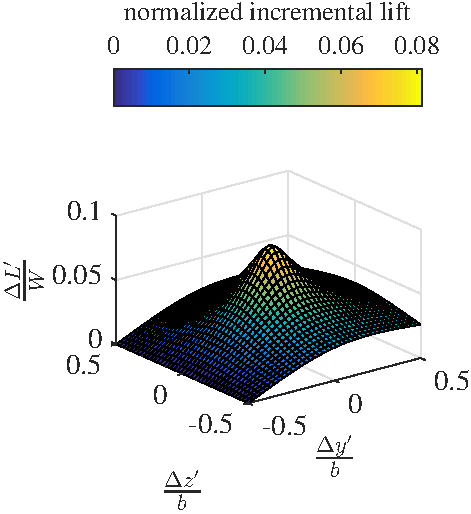
\includegraphics[width=8.4cm]{incrementallift}    % The printed column width is 8.4 cm.
\caption{Normalized incremental lift predicted by modified Horseshoe Vortex Model for $\Delta x' = 2b$. Note that $\Delta x', \Delta y', \Delta z'$ are wingtip to wingtip separations}
\label{fig:HSVMincrementalift}
\end{center}
\end{figure}

A variety of approaches has been proposed to simulate the effects of wake trailing vortices on following UAS, mostly based on modified Horseshoe Vortex Models (HVM) ((!!!citethemall)) or Vortex Lattice methods (VLM) ((!!!citethemall)). For the purpose of this work, a HVM with modified core model presented in (\cite{dogan2005modeling}) is used. It is reported to provide predictions that are in good agreement of both VLM models and wind tunnel measurements while being of great simplicity. In the vertical channel, the model predicts incremental aerodynamic lift perturbations as a function of the separation vector between a UAS and its predecessor, see fig. \ref{fig:HSVMincrementalift}.
A variety of approaches has been proposed to simulate the effects of wake trailing vortices on following UAS, mostly based on modified Horseshoe Vortex Models (HVM) ((citethemall)) or Vortex Lattice methods (VLM) ((citethemall)). For the purpose of this work, a HVM with modified core model presented in (\cite{dogan2005modeling}) is used. It is reported to provide predictions that are in good agreement of both VLM models and wind tunnel measurements while being of great simplicity. The model predicts incremental aerodynamic lift perturbations as a function of the separation vector between a UAS and its predecessor, see fig. \ref{fig:HSVMincrementalift}.

\subsubsection{Atmospheric turbulence}
Atmospheric turbulence time series are generated according to the Dryden turbulence spectrum. The induced velocities are filtered by transfer functions corresponding to closed loop LQR load factor controllers designed for a small UAS ($b=2.6m$).

\subsubsection{Maneuver}

\begin{figure}
\begin{center}
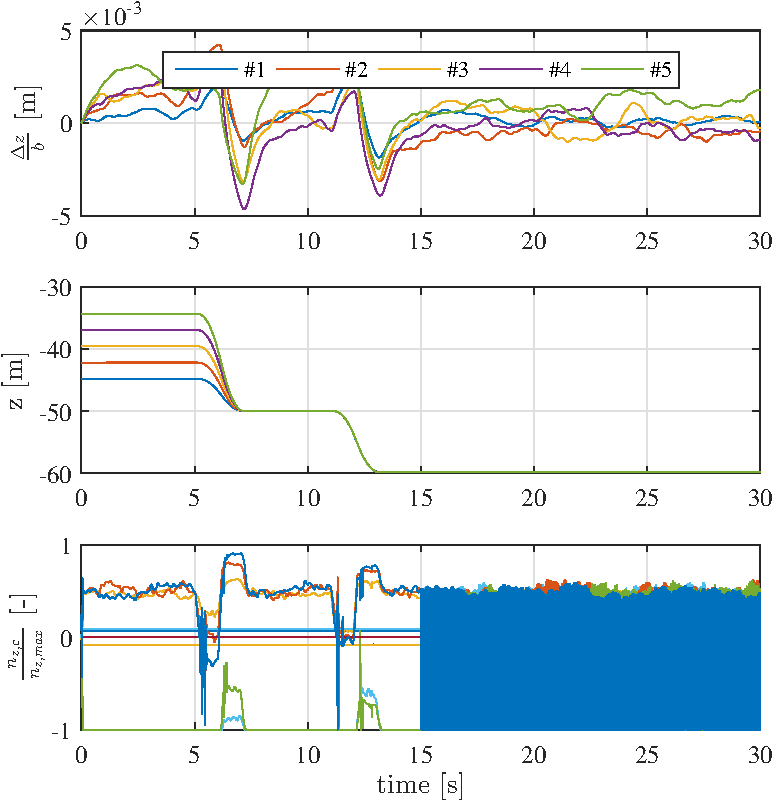
\includegraphics[width=8.4cm]{STSMC-1000Hz-TIMESCALESEPARATION-turbulence=1}    % The printed column width is 8.4 cm.
\caption{CSMC controller $10^{-3} s$ sampling time}
\label{fig:CSMC1000Hz}
\end{center}
\end{figure}

\begin{figure}
\begin{center}
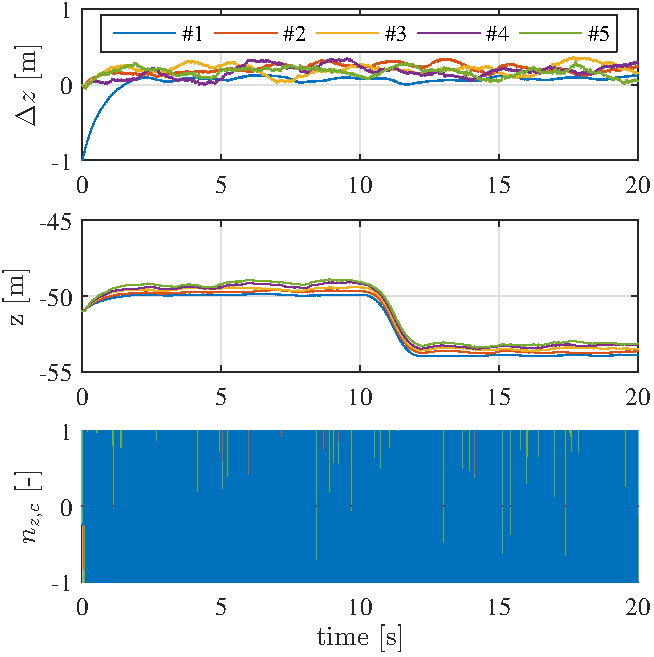
\includegraphics[width=8.4cm]{STSMC-100Hz-TIMESCALESEPARATION-turbulence=1}    % The printed column width is 8.4 cm.
\caption{ CSMC controller $10^{-2} s$ sampling time}
\label{fig:CSMC100Hz}
\end{center}
\end{figure}

\begin{figure}
\begin{center}
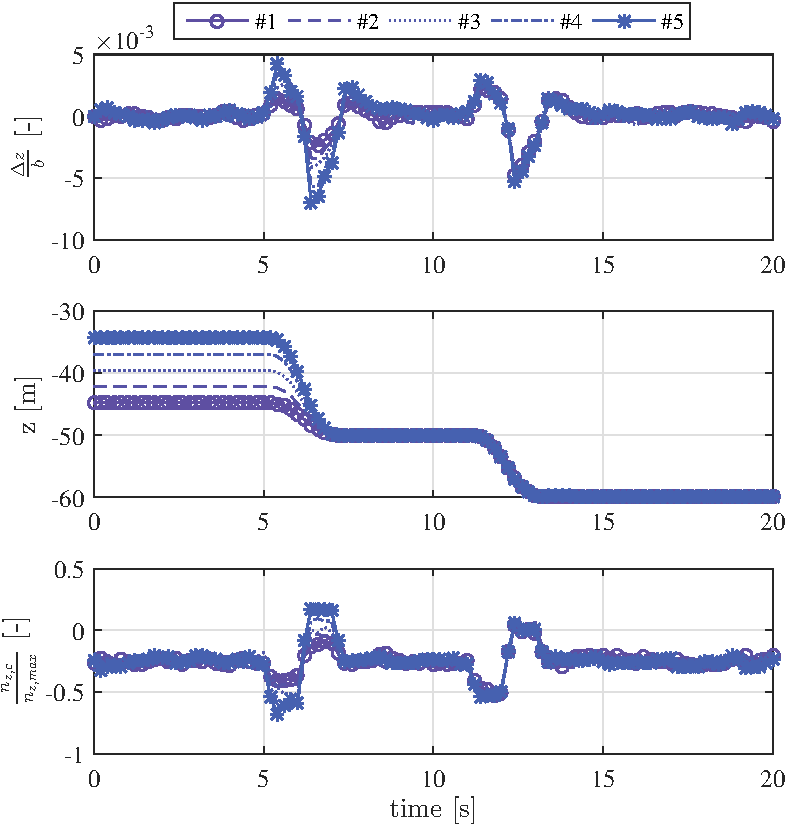
\includegraphics[width=8.4cm]{DSMC-100Hz-TIMESCALESEPARATION-turbulence=1}    % The printed column width is 8.4 cm.
\caption{ DSMC controller $10^{-2} s$ sampling time}
\label{fig:DSMC100Hz}
\end{center}
\end{figure}

\begin{figure}
\begin{center}
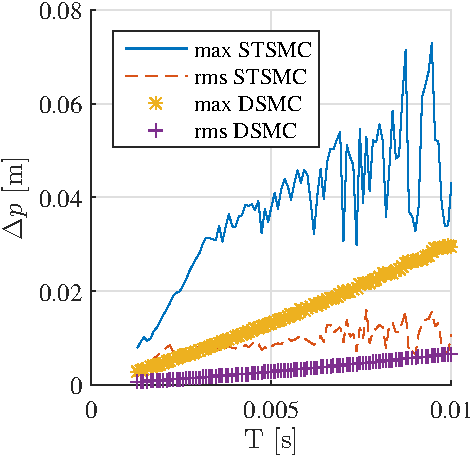
\includegraphics[width=8.4cm]{CSTSMC-DSMC-error-z-samplingtime.pdf}    % The printed column width is 8.4 cm.
\caption{Vertical position error measures vs. controller sampling time for CSTSMC and DSMC}
\label{fig:cst}
\end{center}
\end{figure}

\bibliography{./bibliography/bibliographyPhD}             % bib file to produce the bibliography
                                                     % with bibtex (preferred)
                                                                                                                            % in the appendices.
\end{document}
